\usetikzlibrary{calc}


\newcommand*{\GridSize}{7}

\newcommand*{\ColorCells}[1]{% #1 = list of x/y/color
  \foreach \x/\y/\color/\text in {#1} {
    \node [fill=\color, draw=none, thick, ,minimum size=1cm] 
      at (\x-.5,\GridSize+0.5-\y) [text=white] {\text};
    }%
}%

\definecolor{LightPink}{rgb}{0.92.,0.8,0.84} % bg color, r,g,b <= 


%%%%%


%\listfiles
\scalebox{0.4}{
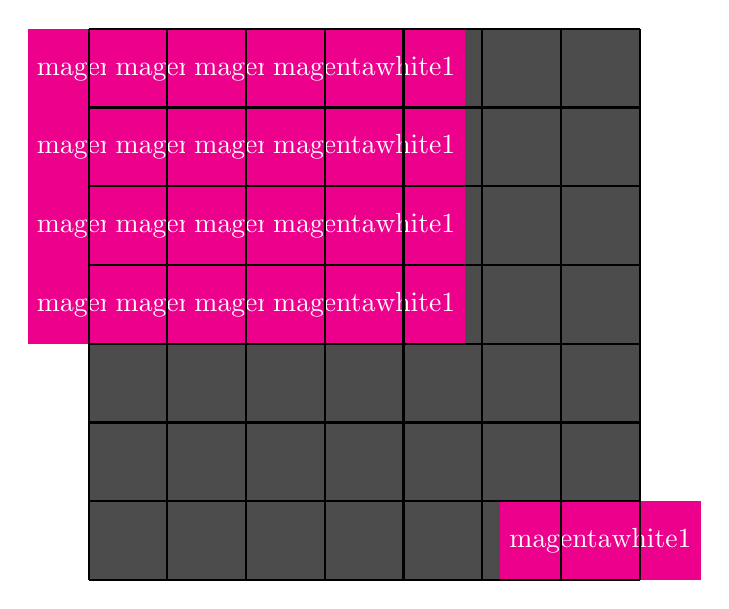
\begin{tikzpicture}
    \begin{scope}[thick,local bounding box=name]
         \fill[black!70](0,0) rectangle (\GridSize,\GridSize);
         \ColorCells{
         1/1/magenta/1,2/1/magenta/1,3/1/magenta/1,4/1/magenta/1,
         1/2/magenta/1,2/2/magenta/1,3/2/magenta/1,4/2/magenta/1,
         1/3/magenta/1,2/3/magenta/1,3/3/magenta/1,4/3/magenta/1,
         1/4/magenta/1,2/4/magenta/1,3/4/magenta/1,4/4/magenta/1,
        7/7/magenta/1}
        \draw (0, 0) grid (\GridSize, \GridSize);
    \end{scope}


\end{tikzpicture}
}